\chapter{Experimental Setup and Matrix Sets}\label{subseq:matrix-sets-and-hardware}


In this study, two matrix sets were used: GRS and SuiteSparse. In our case, the SiteSparse matrix set was, in fact, few matrices downloaded from SuiteSparse Matrix Collection \cite{sparse-matrix-collection:1}, \cite{sparse-matrix-collection:2}. We tried to choose different matrices from the collection with respect to both the number of equations $n$ in a system and ratio $R$ between the number of non-zero elements $nnz$ and the number of equations.\\ 


To generate GRS matrix set, we ran the most common GRS simulations in ATHLET and stopped the simulations somewhere in the middle saving corresponding shifted Jacobian matrices in the PETSc binary format.\\


The main matrix properties as well as matrix sparsity patterns are shown in tables \ref{table:grs-matrix-set}, \ref{table:suite-sparse-matrix-set} and appendix \ref{app:sparsity-patterns}.


\begin{table}[ht]
\small
\centering
\begin{tabular}{|c|c|c|c|c|c|}
\hline
Name     & N       & NNZ      & NNZ / N & \begin{tabular}[c]{@{}c@{}}Approximate\\ Condition\\  Number\end{tabular} & Structure     \\ \hline
pwr-3d   & 6009    & 32537    & 5.4147  & 1.019e+07                                                                 & SYMM-PTRN \\ \hline
cube-5   & 9325    & 117897   & 12.6431 & 1.592e+09                                                                 & SYMM-PTRN \\ \hline
cube-64  & 100657  & 1388993  & 13.7993 & 7.406e+08                                                                 & SYMM-PTRN \\ \hline
cube-645 & 1000045 & 13906057 & 13.9054 & 6.474e+08                                                                 & SYMM-PTRN \\ \hline
k3-2     & 130101  & 787997   & 6.0568  & 1.965e+15                                                                 & SYMM-PTRN \\ \hline
k3-18    & 1155955 & 7204723  & 6.2327  & 1.947e+12                                                                 & SYMM-PTRN \\ \hline
\end{tabular}
\caption{GRS matrix set \textit{(SYMM - symmetric; NON-SYMM - non-symmetric; SYMM-PTRN- non-symmetric but with symmetric sparsity pattern)}}
\label{table:grs-matrix-set}
\end{table}




\begin{table}[ht]
\centering
\small
\begin{tabular}{|c|c|c|c|c|c|c|}
\hline
Name        & N       & NNZ      & NNZ / N & \begin{tabular}[c]{@{}c@{}}Approximate\\ Condition\\ Number\end{tabular} & Structure & Problem                                                      \\ \hline
cant        & 62451   & 4007383  & 64.1684 & 5.082e+05 & SYMM      & -                                                            \\ \hline
consph      & 83334   & 6010480  & 72.1251 & 2.438e+05 & SYMM      & -                                                            \\ \hline
CurlCurl\_3 & 1219574 & 13544618 & 11.1060 & 2.105e+05                                                                & SYMM      & \begin{tabular}[c]{@{}c@{}}Model\\ Reduction\end{tabular}    \\ \hline
Geo\_1438   & 1437960 & 63156690 & 43.9210 & 4.677e+05                                                                 & SYMM      & -                                                            \\ \hline
memchip     & 2707524 & 13343948 & 4.9285  & 1.305e+07                                                                & NON\_SYMM & \begin{tabular}[c]{@{}c@{}}Circuit\\ Simulation\end{tabular} \\ \hline
PFlow\_742  & 742793  & 37138461 & 49.9984 & 5.553e+06                                                                & SYMM      & -                                                            \\ \hline
pkustk10    & 80676   & 4308984  & 53.4110 & 5.589e+02 & SYMM      & Structural                                                   \\ \hline
torso3      & 259156  & 4429042  & 7.0903  & 2.456e+03                                                                      & NON\_SYMM & -                                                            \\ \hline
x104        & 108384  & 8713602  & 80.3956 & 3.124e+05 & SYMM      & Structural                                                   \\ \hline
\end{tabular}
\caption{SuiteSparse matrix set \textit{(SYMM - symmetric; NON-SYMM - non-symmetric; SYMM-PTRN- non-symmetric but with symmetric sparsity pattern)}}
\label{table:suite-sparse-matrix-set}
\end{table}

Approximations of condition numbers were computed by means of Rayleigh–Ritz procedure \cite{rayleigh-ritz-procedure}. GMRES solver, with $1000$ iteration steps, was applied for un-preconditioned systems to generate a Krylov subspace for each matrix. Then, the resulting Hessenberg matrices were used for approximating eigenspaces and the corresponding eigenvalues. The approximations should be treated as lower bound since the algorithm overestimates the smallest eigenvalue.\\


The objective of this study is to find and configure a sparse linear solver which can fulfill all requirements listed above for the GRS matrix set. It is worth pointing out, as it was mentioned in section \ref{sec:athlet-overview}, ATHLET performs many mathematical transformations upon the original system and, finally, generates an approximation of a Jacobian matrix. For that reason, one can assume that GRS matrix set can be structurally different from matrices coming naturally from finite-volume, finite-elements discretization or optimization problems. Therefore, SuiteSparse matrix set was used, from time to time, to examine this statement.\\


Tow different hardware were available for this study. The first machine was the GRS cluster (HW1) which was the main target. Additionally, LRZ CoolMUC-2 Linux cluster (HW2) was used every time when we got some ambiguous results to check whether a problem was hardware, software or algorithm specific. Table \ref{table:hardware-spec} shows a single node specification of both machines.\\


\begin{table}[ht]
\centering
\small
\begin{tabular}{|l|c|c|}
\hline
                    & HW1 (GRS) & HW2 (LRZ Linux) \\ \hline
Architecture        & x86\_64 & x86\_64 \\ \hline
CPU(s)              & 20 &  28 \\ \hline
On-line CPU(s) list & 0-19 &  0-27 \\ \hline
Thread(s) per core  & 1 &  1 \\  \hline
Core(s) per socket  & 10 & 14 \\ \hline
Socket(s)           & 2 &  2 \\ \hline
NUMA node(s)        & 2 &  4 \\ \hline
Model               & 62 &  63 \\ \hline
Model name          & E5-2680 v2 & 
E5-2697 v3 \\ \hline
Stepping            & 4 &  2 \\ \hline
CPU MHz             & 1200.0 &  2036.707 \\ \hline
Virtualization      & VT-x &  VT-x \\ \hline
L1d cache           & 32K &  32K \\ \hline
L1i cache           & 32K &  32K \\ \hline
L2 cache            & 256K &  256K \\ \hline
L3 cache            & 25600K &  17920K \\ \hline
NUMA node0 CPU(s)   & 0-9 &  0-6 \\ \hline
NUMA node1 CPU(s)   & 10-19 &  7-13 \\ \hline
NUMA node2 CPU(s)   & - &  14-20 \\ \hline
NUMA node3 CPU(s)   & - &  21-27 \\ \hline
\end{tabular}
\caption{Hardware specification}
\label{table:hardware-spec}
\end{table}


For this study, OpenMPI implementation of the MPI standard was used because of its open-source license and comprehensive documentation. The library has many options for processes pinning which was quite important for of this study.\\


To make process pinning explicit and deterministic, a python script was developed to generate rank-files automatically based on the number of MPI processes, OpenMP threads per MPI process, the maximum number of processing elements and the number of NUMA domains. The scrip always leaves appropriate gaps between MPI processes to allow each process to fork the corresponding number of threads within a parallel region.\\


\begin{figure}[h!]
\centering
	\begin{tabular}{cc}
			\subfloat[\textit{Spread} mode]{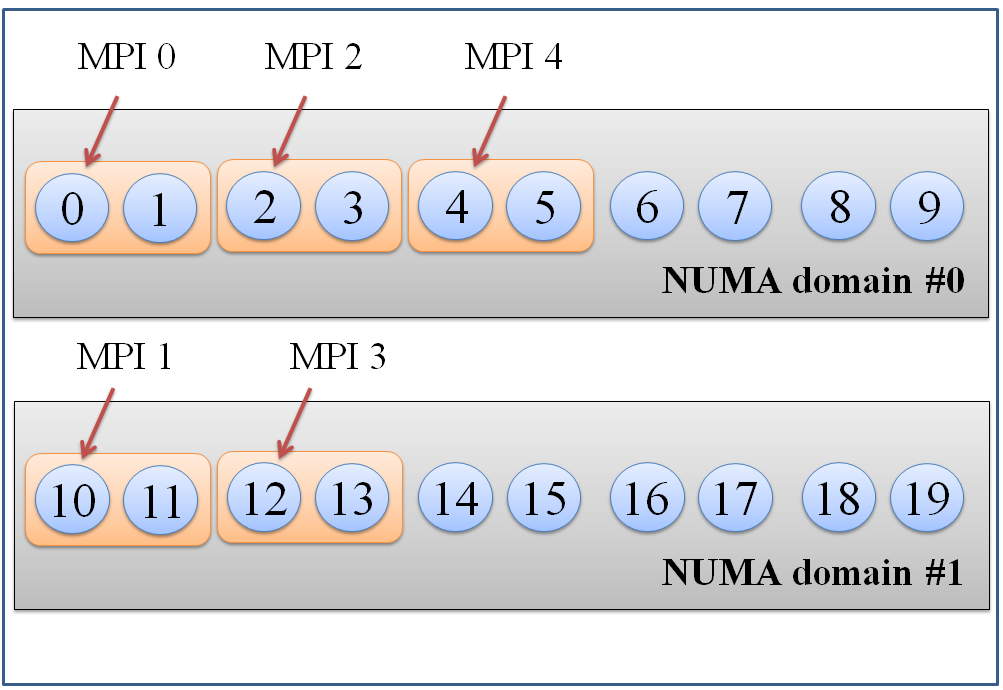
\includegraphics[width=0.45\textwidth]{figures/chapter-2/spread-mode.png}} &
		\subfloat[\textit{Close} mode]{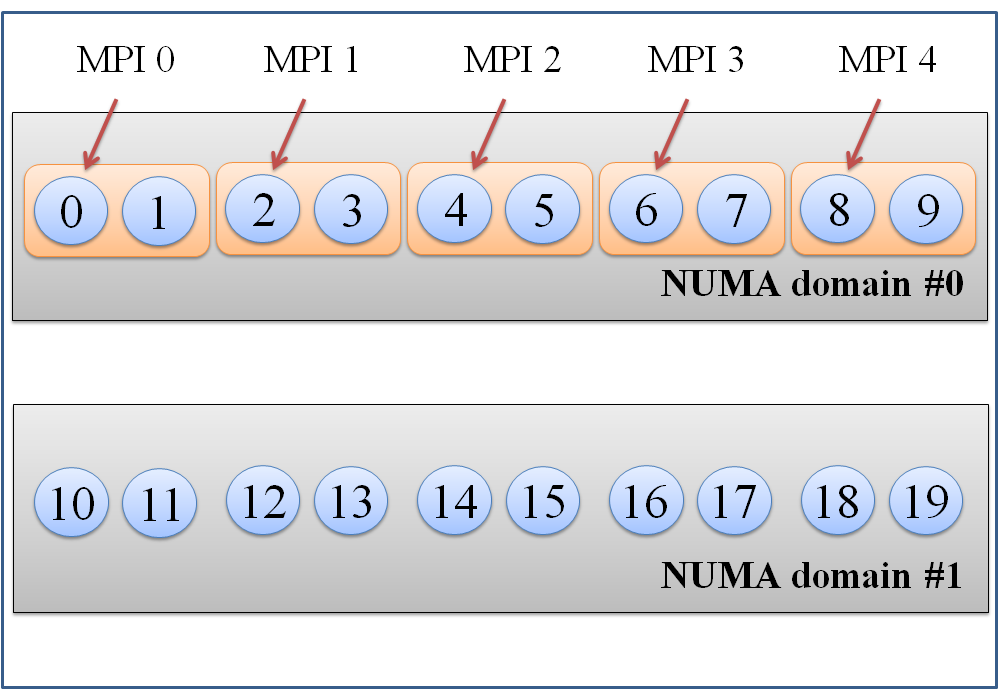
\includegraphics[width=0.45\textwidth]{figures/chapter-2/close-mode.png}} \\
	\end{tabular}
	\caption{An example of process pinning of 5 MPI processes with 2 OpenMP threads per rank in case of HW1 hardware}
	\label{fig:python-script-rankfile-example}
\end{figure}


A rank-file specifies explicit mapping between MPI processes (ranks) and actual processing elements, cores, within a machine. The script has two modes, namely: \textit{spread} and \textit{close}. Given a certain number of ranks, \textit{spread} mode tries to distribute them as spread as possible across multiple available NUMA domains in a round-robin fashion. In contrast to \textit{spread} strategy, \textit{close} one groups ranks as close as possible to keep the maximum number of ranks within a single NUMA domain. Figure \ref{fig:python-script-rankfile-example} shows an example of how these two modes work in case of 5 MPI ranks, 2 OpenMP threads per rank, on a compute node equipped with 20 cores and 2 NUMA domains (HW1).\\


In this study, PETSc 3.10 and OpenMPI 3.1.1 libraries were chosen and compiled with Intel 18.2 compiler.\\